%%%%%%%%%%%%%%%%%%%%%%%%%%%%%%%%%%%%%%%%%
% Beamer Presentation
% LaTeX Template
% Version 1.0 (10/11/12)
%
% This template has been downloaded from:
% http://www.LaTeXTemplates.com
%
% License:
% CC BY-NC-SA 3.0 (http://creativecommons.org/licenses/by-nc-sa/3.0/)
%
%%%%%%%%%%%%%%%%%%%%%%%%%%%%%%%%%%%%%%%%%

%----------------------------------------------------------------------------------------
%	PACKAGES AND THEMES
%----------------------------------------------------------------------------------------

\documentclass{beamer}

\mode<presentation> {

% The Beamer class comes with a number of default slide themes
% which change the colors and layouts of slides. Below this is a list
% of all the themes, uncomment each in turn to see what they look like.

%\usetheme{default}
%\usetheme{AnnArbor}
%\usetheme{Antibes}
%\usetheme{Bergen}
%\usetheme{Berkeley}
%\usetheme{Berlin}
%\usetheme{Boadilla}
%\usetheme{CambridgeUS}
%\usetheme{Copenhagen}
%\usetheme{Darmstadt}
%\usetheme{Dresden}
%\usetheme{Frankfurt}
%\usetheme{Goettingen}
%\usetheme{Hannover}
%\usetheme{Ilmenau}
%\usetheme{JuanLesPins}
%\usetheme{Luebeck}
\usetheme{Madrid}
%\usetheme{Malmoe}
%\usetheme{Marburg}
%\usetheme{Montpellier}
%\usetheme{PaloAlto}
%\usetheme{Pittsburgh}
%\usetheme{Rochester}
%\usetheme{Singapore}
%\usetheme{Szeged}
%\usetheme{Warsaw}

% As well as themes, the Beamer class has a number of color themes
% for any slide theme. Uncomment each of these in turn to see how it
% changes the colors of your current slide theme.

%\usecolortheme{albatross}
%\usecolortheme{beaver}
%\usecolortheme{beetle}
%\usecolortheme{crane}
%\usecolortheme{dolphin}
%\usecolortheme{dove}
%\usecolortheme{fly}
%\usecolortheme{lily}
%\usecolortheme{orchid}
%\usecolortheme{rose}
%\usecolortheme{seagull}
%\usecolortheme{seahorse}
%\usecolortheme{whale}
%\usecolortheme{wolverine}

%\setbeamertemplate{footline} % To remove the footer line in all slides uncomment this line
%\setbeamertemplate{footline}[page number] % To replace the footer line in all slides with a simple slide count uncomment this line

%\setbeamertemplate{navigation symbols}{} % To remove the navigation symbols from the bottom of all slides uncomment this line
}

\usepackage{todonotes}
\usepackage{graphicx} % Allows including images
\usepackage{booktabs} % Allows the use of \toprule, \midrule and \bottomrule in tables

%----------------------------------------------------------------------------------------
%	TITLE PAGE
%----------------------------------------------------------------------------------------

\title[BKG]{Building Knowledge Graphs} % The short title appears at the bottom of every slide, the full title is only on the title page

\author[Data Science]{Lukas Bl{\"u}baum \\ Nick D{\"u}sterhus \\ Monika Werner} % Your name
\institute[UPB] % Your institution as it will appear on the bottom of every slide, may be shorthand to save space
{
University of Paderborn \\ % Your institution for the title page
\medskip
\textit{https://github.com/LukasBluebaum/BKG} % Your email address
}
\date{June 21, 2018} % Date, can be changed to a custom date

\begin{document}

\begin{frame}
\titlepage % Print the title page as the first slide
\end{frame}

\begin{frame}
\frametitle{Overview} % Table of contents slide, comment this block out to remove it
\tableofcontents % Throughout your presentation, if you choose to use \section{} and \subsection{} commands, these will automatically be printed on this slide as an overview of your presentation
\end{frame}

%----------------------------------------------------------------------------------------
%	PRESENTATION SLIDES
%----------------------------------------------------------------------------------------

%------------------------------------------------
\section{Preprocessing (Cleaning and Coreference Resolution)} % Sections can be created in order to organize your presentation into discrete blocks, all sections and subsections are automatically printed in the table of contents as an overview of the talk
%------------------------------------------------

\begin{frame}
\frametitle{Extraction and cleaning of text from Wikipedia Dump}
\begin{block}{Foundation}
	Wikipedia Dump consisting of plain text without markup, infoboxes or chapter subdivision 
\end{block}
\begin{itemize}
	\item Using regular expressions to remove unnecessary URLs, parentheses, whitespace, nullchar, symbols
	\item WikiCleaner class using Writer and Reader Threads for faster cleaning
\end{itemize}
\end{frame}

%------------------------------------------------

%------------------------------------------------

\begin{frame}
\frametitle{Extraction and cleaning of text from Wikipedia Dump}
\begin{columns}[c] % The "c" option specifies centered vertical alignment while the "t" option is used for top vertical alignment

\column{.5\textwidth} % Left column and width
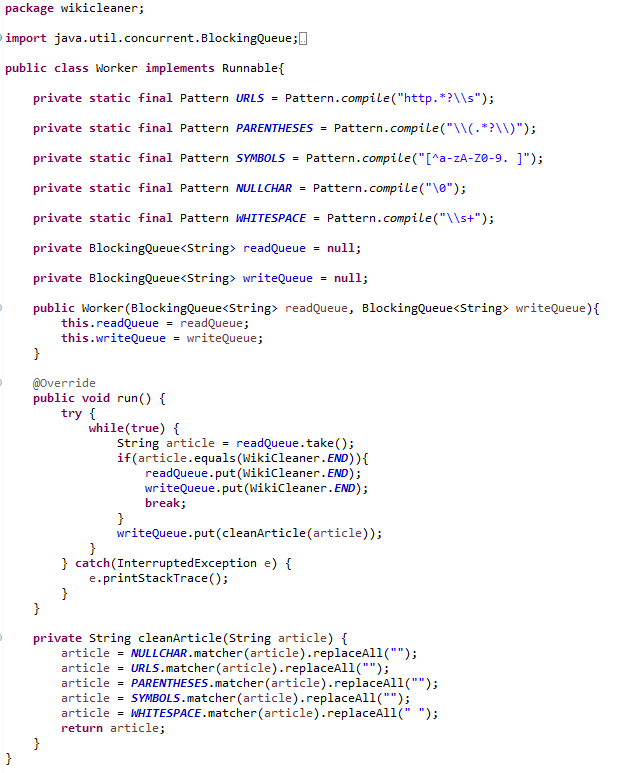
\includegraphics[scale=0.35]{Worker.PNG}

\column{.5\textwidth} % Right column and width
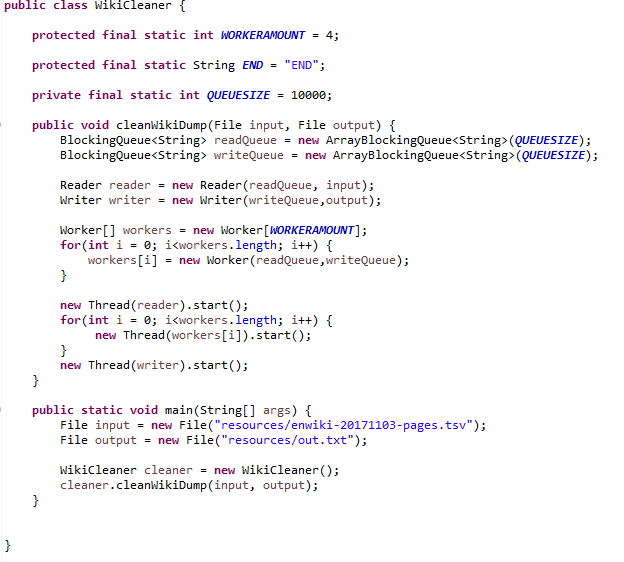
\includegraphics[scale=0.4]{WikiCleaner.PNG}

\end{columns}
\end{frame}

\begin{frame}
\frametitle{Coreference Resolution}
\begin{itemize}
	\item Stanford NLP CoreRef to find the representative mention
	\item Replace pronouns and possessive pronouns
\end{itemize}
\begin{example}[]
	\begin{itemize}
		\item John met Judy in 1960. He married her during his college year.
		\item[] $\Rightarrow$ John met Judy in 1960. John married Judy during John's college year.
	\end{itemize}
\end{example}
\end{frame}

%------------------------------------------------


%------------------------------------------------
\section{Named Entity Recognition}
%------------------------------------------------

\begin{frame}
\frametitle{Named Entity Recognition}
\begin{columns}[c]
\column{.5\textwidth} % Left column and width
\begin{itemize}
	\item Requesting Spotlight Demo and parsing JSON response to Entity class
\end{itemize}
\column{.5\textwidth} % Left column and width	
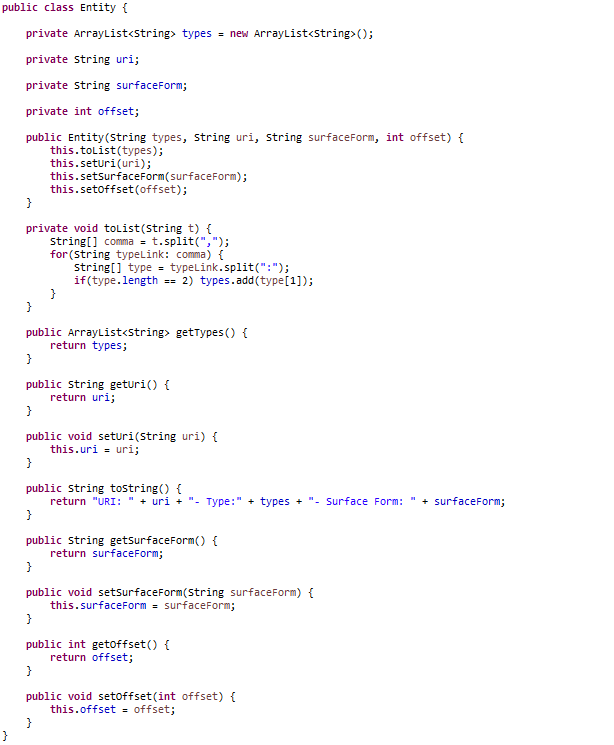
\includegraphics[scale=0.4]{Entity.PNG}
\end{columns}
\end{frame}

%------------------------------------------------

%------------------------------------------------
\section{Entity Disambiguation}
%------------------------------------------------

\begin{frame}
\frametitle{Entity Disambiguation}
\begin{block}{Frameworks}
\begin{itemize}
	\item Spotlight: Integrated disambiguation with two approaches: 
	\begin{itemize}
		\item The information (context) next to a candidate's surface forms is used to find the most likely disambiguation. The best match determines the selection.
		\item Weigh words on their ability to disambiguate between the resources
	\end{itemize}
	\item[] \cite{p2}
	\item Fox: AGDISTIS
\end{itemize}
\end{block}
\begin{itemize}
	\item[] $\Rightarrow$ Done by given Frameworks
\end{itemize}

\end{frame}

%------------------------------------------------

%------------------------------------------------
\section{Relation Extraction}
%------------------------------------------------

\begin{frame}
\frametitle{Relation Extraction}
\begin{itemize}
	\item Two ways of extracting Relations:
	\begin{itemize}
		\item Fox in 're' mode, performing entity recognition as well as relation extraction
		\begin{itemize}
			\item Saving triple statements
		\end{itemize}
		\item Our RelationExtraction Method using OpenIE and Spotlight 
	\end{itemize}
	\item Limited to the first part of each article (summarizes the facts)
\end{itemize}
\end{frame}

%------------------------------------------------

\begin{frame}
\frametitle{Relation Extraction: Fox}

\begin{figure}
	\begin{center}
		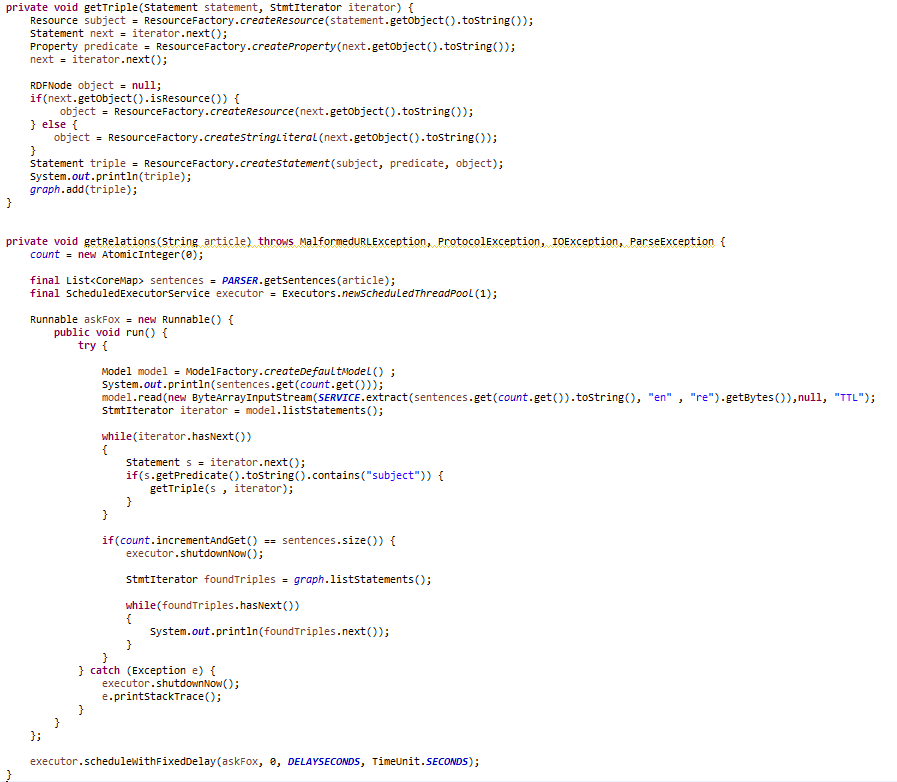
\includegraphics[scale=0.38]{FoxExtraction.PNG}
	\end{center}
\end{figure}
\end{frame}

%------------------------------------------------

\begin{frame}
\frametitle{Relation Extraction: Own Approach}
\begin{itemize}
	\item Parsing ontology and creating a list of properties
	\item Using Spotlight for NER, so we can run it concurrent to Fox
	\item Using Stanford CoreNLP 
	\begin{itemize}
		\item experimented with different approaches to find relations given two entities (search algorithms on dependency trees, semanticGraph)
		\item decided to use OpenIE
	\end{itemize}
\end{itemize}
\end{frame}

%------------------------------------------------

\begin{frame}
\frametitle{Relation Extraction: OpenIE }
\begin{itemize}
	\item Splitting sentences into shorter fragments, appeal to natural logic to maintain context
	\item Traverse dependency parse tree recursively \cite{p1}
	\item Disadvantage in our case: have to filter for entity to entity relation 
	\item After finding the binary relation (OpenIE Triple) between entities: Map them to DBpedia ontology
\end{itemize}
\end{frame}

%------------------------------------------------

\begin{frame}
\frametitle{Relation Extraction: OpenIE }
\begin{itemize}
	\item Parse DBpedia properties to Java objects
	\item Search for a valid property (check domain and range)
	\item Map relation to keywords to find proper property 
	\item Write triple to graph
\end{itemize}
\end{frame}

%------------------------------------------------

%------------------------------------------------
\section{Architecture}
%------------------------------------------------

\begin{frame}
\frametitle{Architecture}
\begin{center}
	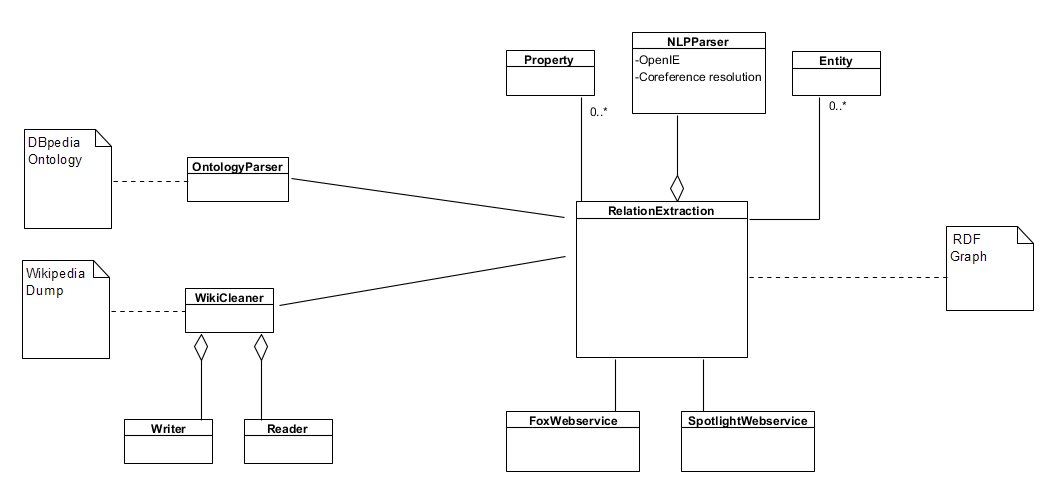
\includegraphics[scale=0.43]{architecture.PNG}
\end{center}
\end{frame}

%------------------------------------------------

%------------------------------------------------
\section{Upcoming Tasks}
%------------------------------------------------

\begin{frame}
\frametitle{Upcoming Task}
\begin{itemize}
	\item Already able to build a knowledge graph, but thinking about further improvements for our own relation extraction
	\begin{itemize}
		\item e.g. more keywords / heuristics for finding the best property
		\item e.g. find entity to literal relations 
		\item long runtime due to response time of Fox/Spotlight and delay for scheduling Fox/Spotlight requests
		\item[] $\Rightarrow$ avoid running it before all improvements are made
	\end{itemize}
	\item Benchmarking as soon as we are pleased with the result (whether improvements are needed)
\end{itemize}
\end{frame}

%------------------------------------------------

\begin{frame}
\frametitle{References}
\footnotesize{
	\begin{thebibliography}{99} % Beamer does not support BibTeX so references must be inserted manually as below
		\bibitem[Mendes, Jakob, García-Silva, Bizer, 2011]{p2} Pablo N. Mendes, Max Jakob, Andrés García-Silva and Christian Bizer (2011)
		\newblock DBpedia Spotlight: Shedding Light on the Web of
		Documents
		\newblock \emph{
			Proceedings of the 7th International Conference on Semantic Systems (I-Semantics) } 3.
	\end{thebibliography}
	\begin{thebibliography}{99} % Beamer does not support BibTeX so references must be inserted manually as below
		\bibitem[Angeli, Premkumar, Manning, 2015]{p1} Gabor Angeli, Melvin Johnson Premkumar, and Christopher D. Manning (2015)
		\newblock Leveraging Linguistic Structure For Open Domain Information
		Extraction
		\newblock \emph{
			In Proceedings of the Association of Computational Linguistics (ACL) } 2.
	\end{thebibliography}
}
\end{frame}

\begin{frame}
\frametitle{Relation Extraction 1.1 - Entity to Literal Relation}
\begin{example}[]
	\begin{itemize}
		\item \textit{Multiple Sentences (as many as Spotlight can handle):} \\
		\begin{itemize} \item Obama was born on August 4, 1961, at Kapiolani Medical Center for Women and Children in Honolulu, Hawaii. He graduated from Havard University.
		\end{itemize}
		\item Coreference Resolution:  \begin{itemize} \item Obama was born on August 4 , 1961 , at Kapiolani Medical Center for Women and Children in Honolulu , Hawaii . Obama graduated from Havard University. 
		\end{itemize}
	\item Binary Relation Extraction:  \begin{itemize} \item First sentence: Obama - be bear on - August 4 1961. (among others)
    \item Second sentence: Obama - graduate from - Havard Law school (among others)
	\end{itemize}	 
	\end{itemize}
\end{example}
\end{frame}
%------------------------------------------------
\begin{frame}
\frametitle{Relation Extraction 1.2 - Entity to Literal Relation}
\begin{example}
	\begin{itemize}
	\item \textit{Named Entity Recognition and mapping surface form back to sentences} \\
	\begin{itemize} \item \underline{Obama} was born on August 4, 1961, at \underline{Kapiolani} Medical Center for Women and Children in \underline{Honolulu}, \underline{Hawaii}. \underline{Obama} graduated from \underline{Havard University} .
	\end{itemize}
	\item Enity to literal extraction: Obama - be bear on - August 4 1961. \begin{itemize} \item Search for entity in subject of the binary relations. \\ $\Rightarrow$ Obama (Types: Person, ...) 
	\item Search for literal in object: $\Rightarrow$ detects numbers 
	\item Search if object contains a date if not extract single literal: \\ $\Rightarrow$ detects month + numbers (date found)
	\item Convert to dateformat: $\Rightarrow$  1961-08-04
	\item Map relation to property: keyword: bear  $\Rightarrow$ dbo:birthDate (Domain: Person Range: xsd:date)
	\item write dbo:Barack\_Obama dbo:birhtDate "1961-08-04"\textasciicircum{}\textasciicircum{}xsd:date to graph.
	\end{itemize}		 
\end{itemize}
\end{example}
\end{frame}
\begin{frame}
\frametitle{Relation Extraction 1.3 - Entity to Entity Relation}
\begin{example}
	\begin{itemize}
		\item \textit{Named Entity Recognition and mapping surface form back to sentences} \\
		\begin{itemize} \item \underline{Obama} was born on August 4, 1961, at \underline{Kapiolani} Medical Center for Women and Children in \underline{Honolulu}, \underline{Hawaii}. \underline{Obama} graduated from \underline{Havard University} .
		\end{itemize}
		\item Enity to entity extraction: Obama - graduate from - Havard University \begin{itemize} \item Search for entity in subject and in object of the binary relations. \\ $\Rightarrow$ Obama (Types: Person, ...), Hardvard University (Type: EducationalInstitution )
			\item Iterate over all properties with given domain and range
			\item Map relation to property: \\ keyword: graduate $\Rightarrow$ dbo:almaMater
			\item write dbo:Barack\_Obama dbo:almaMater dbo:Havard\_University to graph.
		\end{itemize}		 

	\end{itemize}
\end{example}
\end{frame}


\end{document} 